\documentclass[10pt, aspectratio=169, compress, protectframetitle, handout]{beamer}
\usepackage[italian]{babel}
\usepackage{appendixnumberbeamer}
% handout to deactivate \uncover
% usetitleprogressbar might be needed
%\usepackage{beamerprosper}
\usepackage{comment}
% Load BEFORE the theme
\usepackage{ulem}
\usepackage{courier}
\renewcommand*\familydefault{\ttdefault} %% Only if the base font of the document is to be typewriter style. WOW!
\usepackage[T1]{fontenc}

\usetheme[progressbar=frametitle,block=fill,numbering=fraction]{metropolis}
\setbeamercolor{frametitle}{bg=white, fg=}
\setbeamertemplate{blocks}[rounded][shadow=true]
%\setbeamertemplate{note page}[plain]
%\setsansfont[
%     Extension      = .otf,
%     UprightFont    = *-Light,
%     ItalicFont     = *-LightItalic,
%     BoldFont       = *-Regular,
%     BoldItalicFont = *-RegularItalic
% ]{FiraSans}
%\setmonofont[
%     Extension   = .otf,
%     UprightFont = *-Regular,
%     BoldFont    = *-Medium
%]{FiraMono}


\newcommand{\putbg}{\usebackgroundtemplate{
\includegraphics[width=\paperwidth,height=\paperheight]{background-vector_169}}}
\newcommand{\putbgdark}{\usebackgroundtemplate{
\includegraphics[width=\paperwidth,height=\paperheight]{background-vector-dark_169}}}

\usepackage{multirow}
\usepackage{multicol}
\usepackage{booktabs}
\usepackage[export]{adjustbox}
\usepackage{boldline}
%\usepackage[]{enumitem}
\usepackage{marvosym}
\usepackage{caption}
\usepackage{subcaption}

\usepackage{datetime}

\usepackage{textpos}
% Fixes bad positioning of hats
\usefonttheme{professionalfonts}%[onlymath]{serif}
\usepackage{siunitx}
\usepackage{dcolumn}
\newcolumntype{d}[1]{D{.}{.}{#1}}
\DeclareSIUnit\atomicunit{a.u.}
\DeclareSIUnit\rydberg{Ry}
%\usepackage{braket}
%\usepackage{cancel}
\PassOptionsToPackage{hyphens}{url}\usepackage{hyperref} % to break the links
%\usepackage{svg} # \includesvg
\usepackage{ragged2e}

%%% Bibliografia
\usepackage[autostyle]{csquotes}
\usepackage[backend=biber]{biblatex}
\addbibresource{biblio.bib}


%%% Metadati
\graphicspath{{figures/PNG/}{figures/PDF/}{figures/}}
\newdateformat{monthyear}{\monthname[\THEMONTH] \THEYEAR}
\title{\vspace*{1.5cm}Information in our era}
\subtitle{A project for the \textit{Data Visualization} course}
\date{26th February 2021}
\author{Angela Carraro, Claudia Dorigo, Nicolas Solomita, Alice Vegliach}
\institute{\scshape DSSC - UniTS
\vfill

\includegraphics[valign=c, height=0.7cm]{logo_dssc_alt}
\hspace*{0.5cm}

\includegraphics[valign=c, height=0.75cm]{Logo_units_blu}
}

\addtobeamertemplate{frametitle}{}{%
\begin{textblock*}{100mm}(0.90\textwidth,-0.94cm)

\includegraphics[valign=c, height=0.4cm]{logo_dssc_alt_white}

\includegraphics[valign=c, height=0.45cm]{Logo_units_white}
\end{textblock*}}

\begin{document}

{\putbg\maketitle}

%\begin{frame}{Contents}
%	\tableofcontents
%\end{frame}

\begin{frame}{Topic and data introduction}
	
    \begin{description}
        \item[\alert{\textbf{Topic}}]
       % \justifying
        Some aspects of our relationship with the \alert{infosphere} (i.e. the set of media and the information they spread) and how it changed with the rise of the Internet.
        \item[\alert{\textbf{Data}}]
        % about Italian people and their selection criteria of the media 
        We use the results of a survey conducted by UNISOB media lab in 2018 which investigates habits and opinions of Italian people about information sources and media.\\
        %about the habits and opinions of Italian people with respect to the media. \\
        \href{https://www.unisob.na.it/eventi/pdf/20180720.pdf}{\color{blue}\underline{Link to the Infosphere report}}.
        % about the criteria Italian people use to choose the information sources.
        % that/which investigates habits and opinions of Italian people about information sources and media.
    \end{description}
	
\end{frame}

\begin{frame}{Addressed questions}
	
    %\alert{Questions}.
    \begin{enumerate}
    \item How the spread of the Internet influenced the way we get informed?
    \item Do we really trust our most used information sources?
    \item Are we able to recognize a fake news?
    \end{enumerate}
	
\end{frame}


{
\usebackgroundtemplate{
    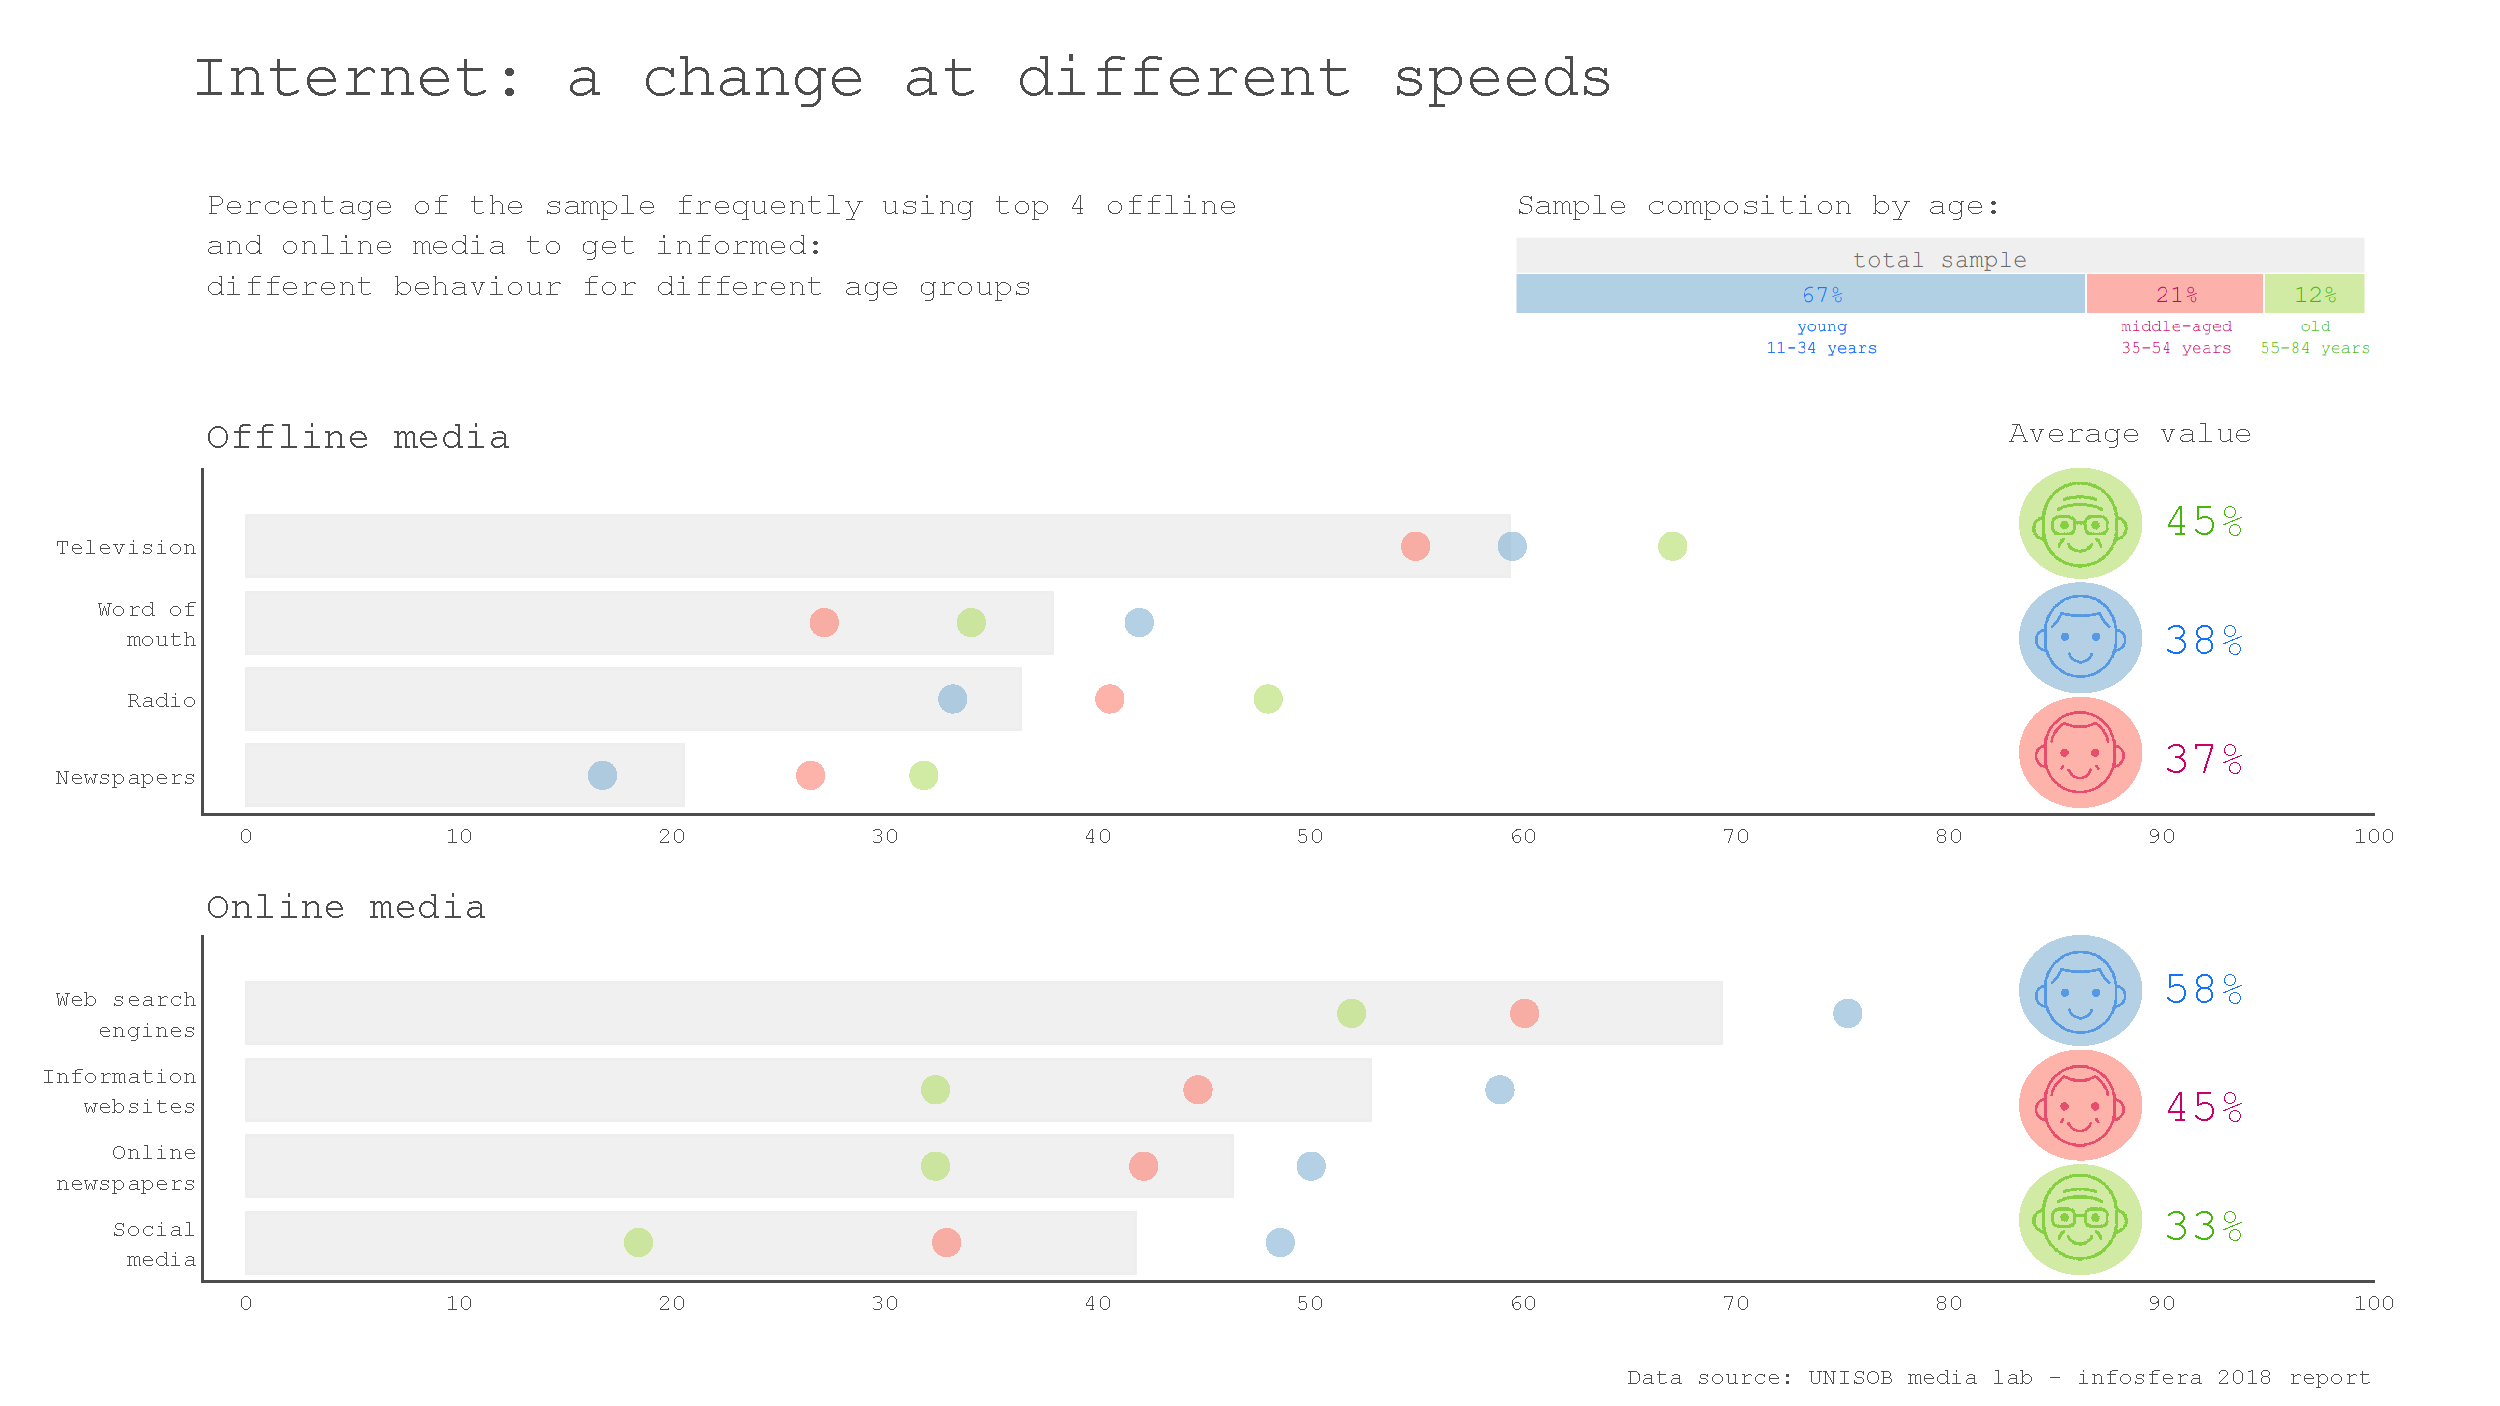
\includegraphics[width=\paperwidth]{graphs/claudia_plot.pdf}
    }
\begin{frame}[plain]
\end{frame}
}

{
\usebackgroundtemplate{
    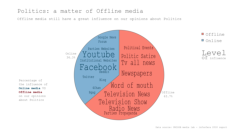
\includegraphics[width=\paperwidth]{graphs/alice_piechart.pdf}
}
\begin{frame}[plain]
\end{frame}
}

{
\usebackgroundtemplate{
    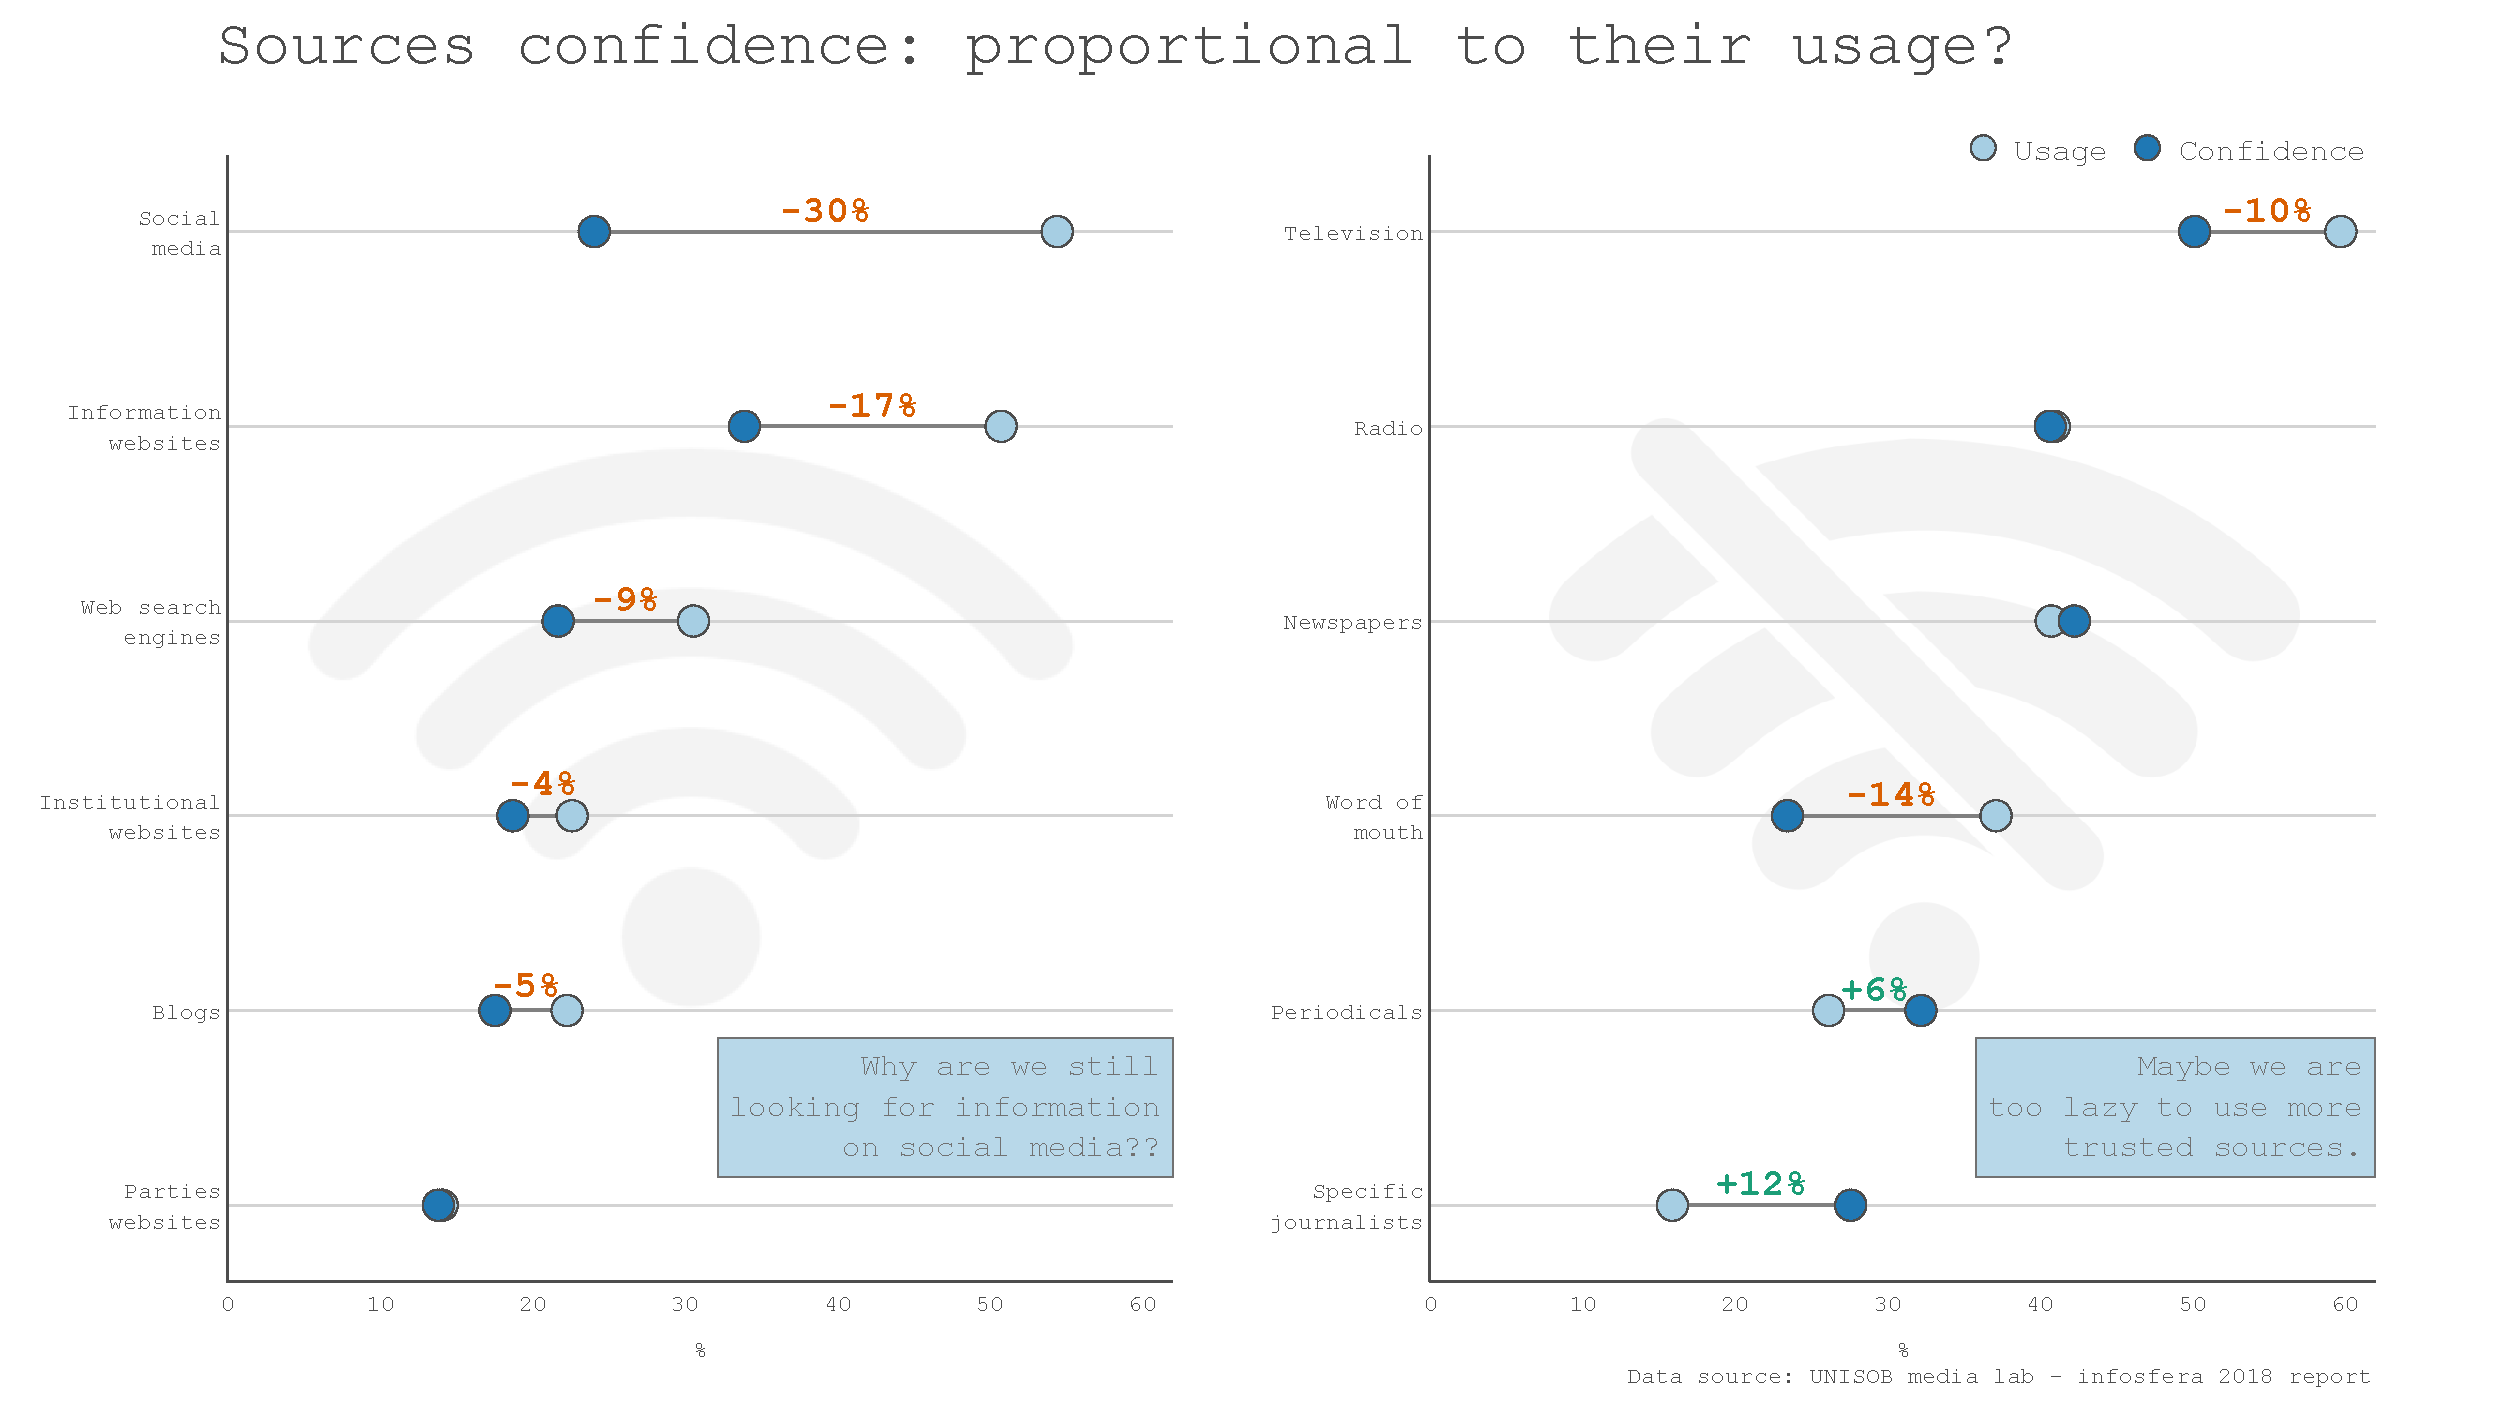
\includegraphics[width=\paperwidth]{graphs/nicolas_plot.pdf}
}
\begin{frame}[plain]
\end{frame}
}


{
\usebackgroundtemplate{
    \leavevmode
    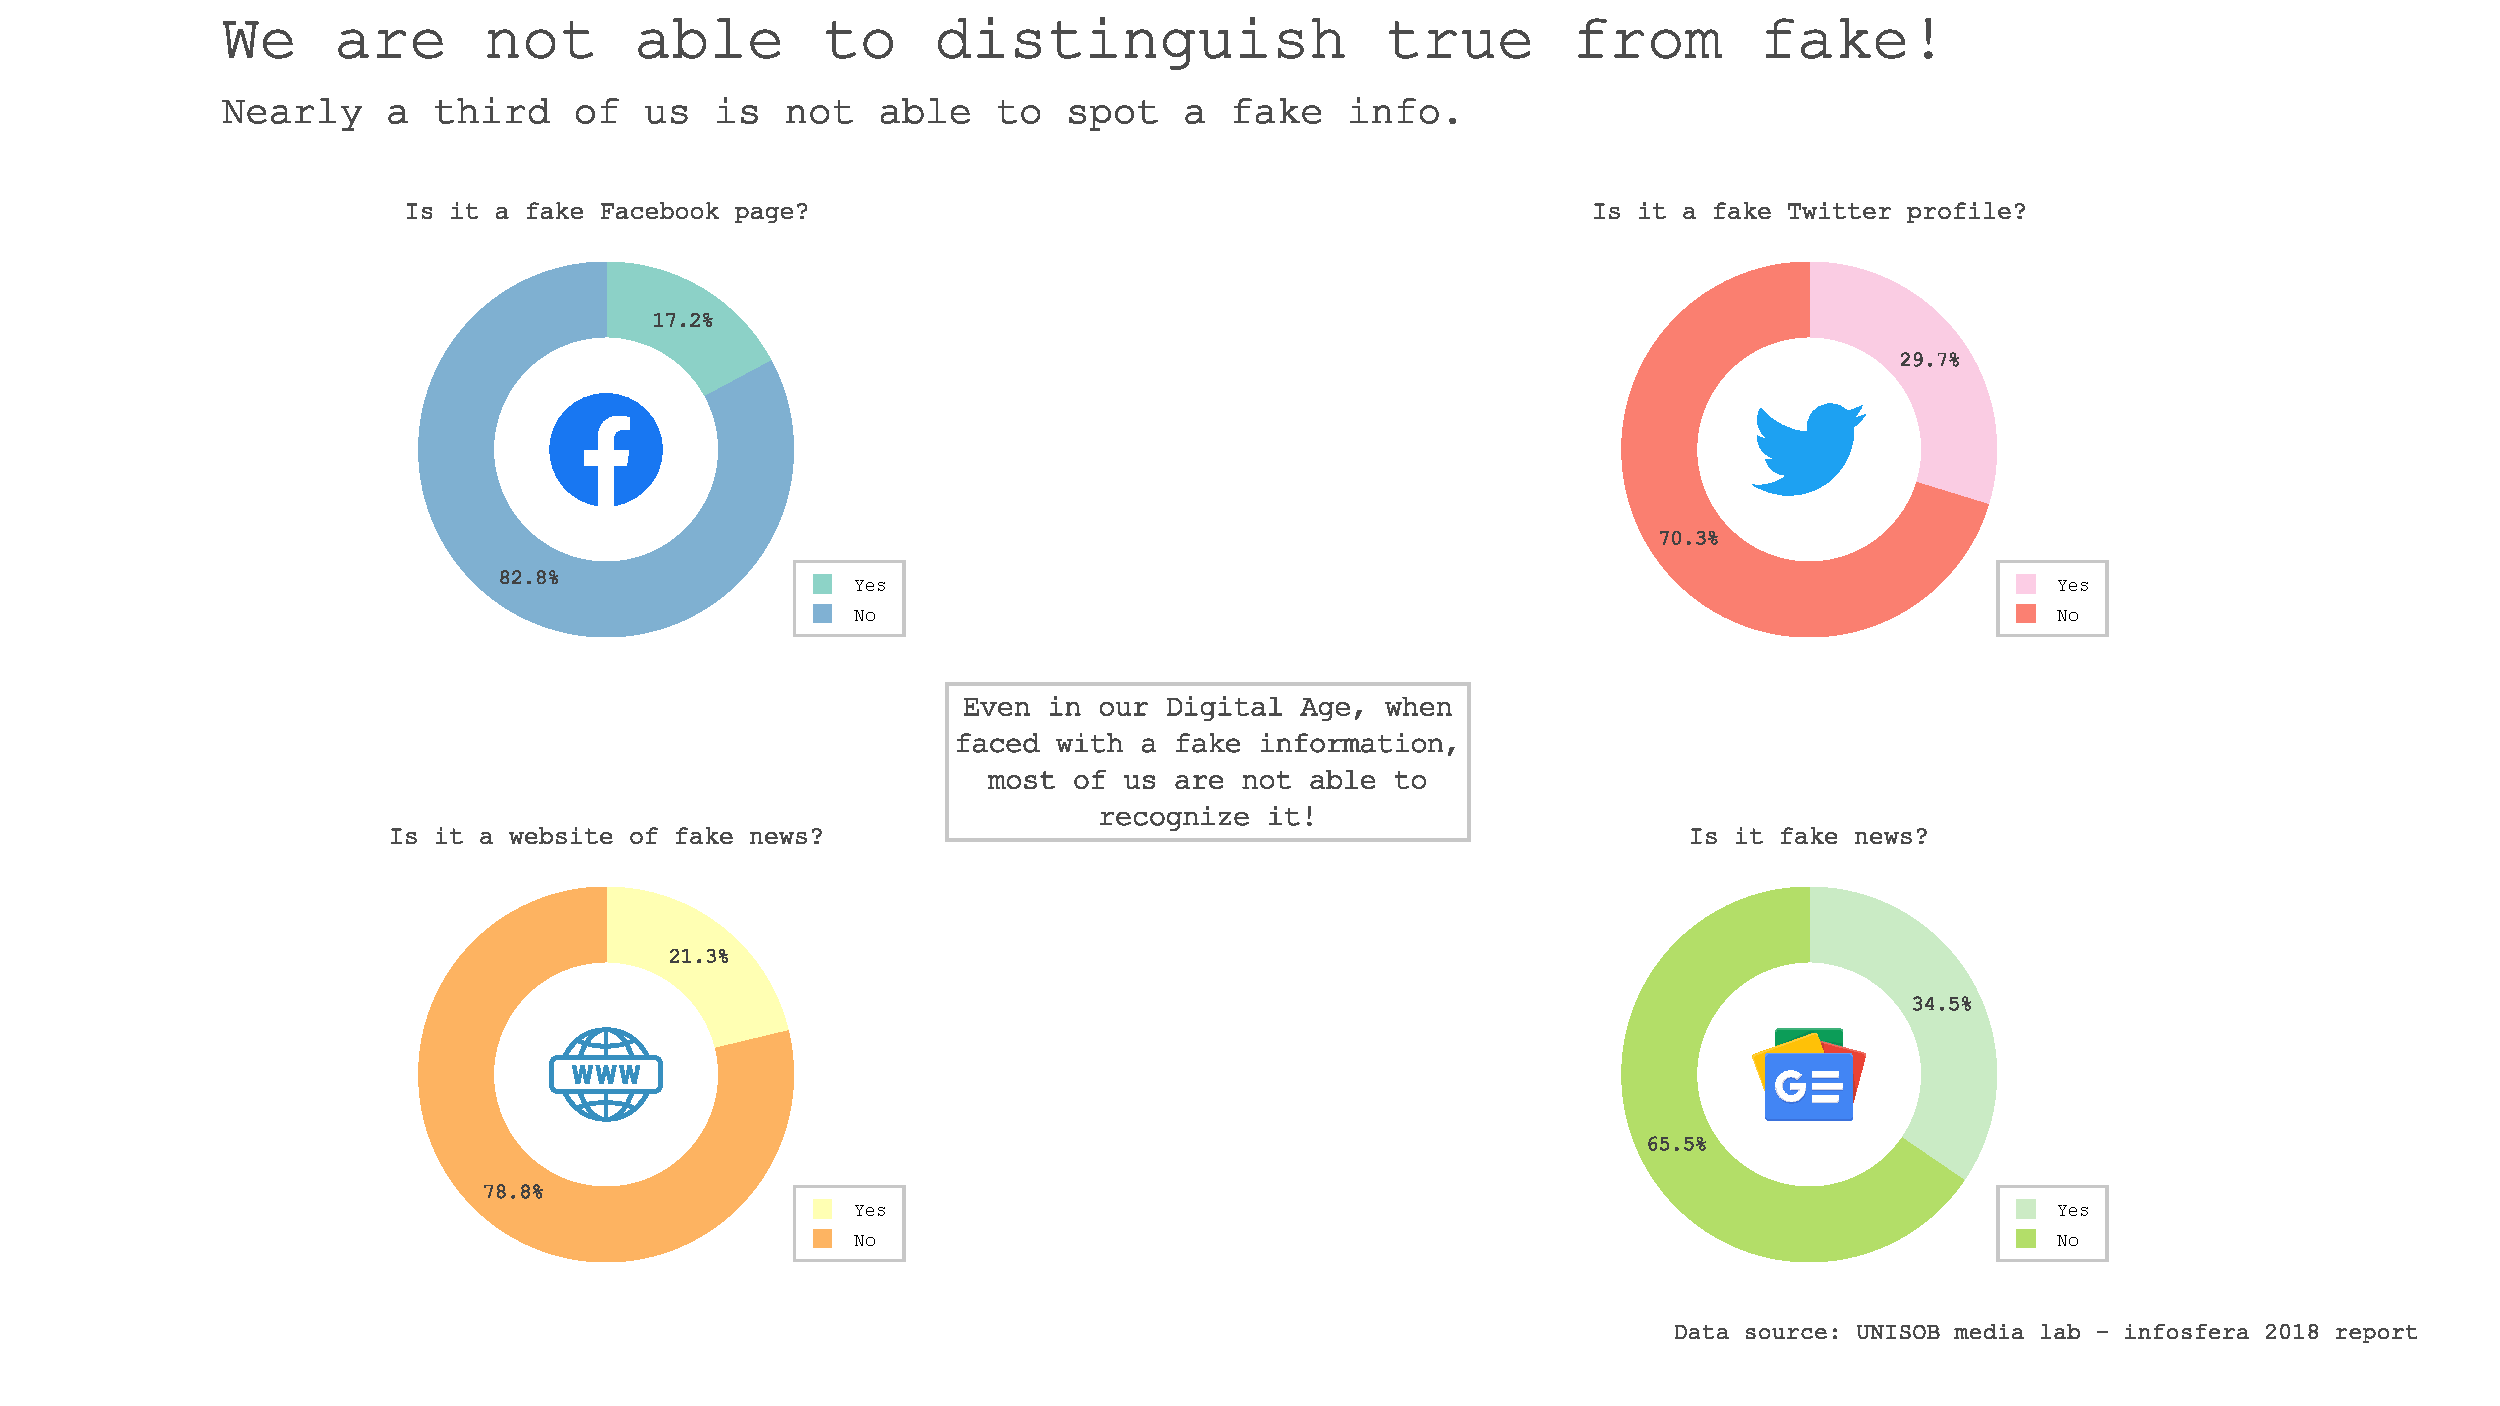
\includegraphics[width=\paperwidth]{graphs/fig_final.pdf}
    }
\begin{frame}[plain]
%\begin{figure}[htbp]
%  \centering
%  \includesvg{graphs/composition.svg}
%\end{figure}
\end{frame}
}

\begin{frame}{Individual contributions}

    {\Huge\uncover<+->{\Ladiesroom}}{\Huge\uncover<+->{\Ladiesroom}}{\Huge\uncover<+->{\Ladiesroom}}{\Huge\uncover<+->{\Gentsroom}} \alert{\textbf{Everybody}} Choice of the dataset and the questions, revision of the plots.

    {\Huge\uncover<+->{\Ladiesroom}} \alert{\textbf{Claudia}} Internet: a change at different speeds
    
    {\Huge\uncover<+->{\Ladiesroom}} \alert{\textbf{Alice}} Online media \& Politics
    
    {\Huge\uncover<+->{\Gentsroom}} \alert{\textbf{Nicolas}} Sources confidence: proportional to their usage?
    
    {\Huge\uncover<+->{\Ladiesroom}} \alert{\textbf{Angela}} Distinguish true from fake

\end{frame}

%\begin{frame}{Considerations}

%    We all used this color scheme from \href{https://colorbrewer2.org/?type=qualitative&scheme=Set3&n=12}{\color{blue}\underline{COLORBREWER 2.0}}.
    
%    We used this tool (\href{https://gka.github.io/palettes/}{\color{blue}\underline{link}}) to check that all the colours we used were color-blind safe.

%\end{frame}


{\putbgdark
\begin{frame}[standout]
	\begin{center}
		\Large \uncover<+->{Thank you for your attention!}
		
		\Huge\uncover<+->{\Smiley}
	\end{center}
\end{frame}
}

%\begin{frame}[standout]
%	Questions?
%\end{frame}
%
%\appendix
%
%{\putbg
%\section{Backup slides}
%}
%
%\begin{frame}[allowframebreaks]{Backup}
%
%	Things
%	
%\end{frame}
%
%
%\begin{frame}[allowframebreaks]{Referenze}
%
%	\nocite{*}
%	\printbibliography
%
%\end{frame}

\end{document}
